\documentclass{ximera}

\title{On different degrees of smallness}

\begin{document}
\begin{abstract}
\end{abstract}
\maketitle

We shall find that in our processes of calculation we
have to deal with small quantities of various degrees
of smallness.

We shall have also to learn under what circumstances
we may consider small quantities to be so minute
that we may omit them from consideration. Everything
depends upon relative minuteness.

Before we fix any rules let us think of some
familiar cases. There are $60$ minutes in the hour,
$24$ hours in the day, $7$ days in the week. There are
therefore $1440$ minutes in the day and $10080$ minutes
in the week.

Obviously $1$ minute is a very small quantity of time compared with a
whole week. Indeed, our forefathers considered it small as compared
with an hour, and called it ``one minute,'' meaning a minute
fraction---namely one sixtieth---of an hour. When they came to require
still smaller subdivisions of time, they divided each minute into $60$
still smaller parts, which, in Queen Elizabeth's days, they called
``second minutes'' (\textit{i.e.:}~small quantities of the second order of
minuteness). Nowadays we call these small quantities

of the second order of smallness ``seconds.'' But few people know
\textit{why} they are so called.

Now if one minute is so small as compared with a whole day, how much
smaller by comparison is one second!

Again, think of a farthing as compared with a sovereign: it is barely
worth more than $\frac{1}{1000}$ part.  A farthing more or less is of
precious little importance compared with a sovereign: it may certainly
be regarded as a \textit{small} quantity. But compare a farthing with
£$1000$: relatively to this greater sum, the farthing is of no more
importance than $\frac{1}{1000}$ of a farthing would be to a
sovereign. Even a golden sovereign is relatively a negligible quantity
in the wealth of a millionaire.

Now if we fix upon any numerical fraction as constituting the
proportion which for any purpose we call relatively small, we can
easily state other fractions of a higher degree of smallness. Thus if,
for the purpose of time, $\frac{1}{60}$ be called a \textit{small}
fraction, then $\frac{1}{60}$ of $\frac{1}{60}$ (being a
\textit{small} fraction of a <em>small</em> fraction) may be regarded
as a \textit{small quantity of the second order} of smallness. (The
mathematicians talk about the second order of ``magnitude''
(\textit{i.e.:} greatness) when they really mean second order of
<em>smallness</em>.  This is very confusing to beginners.)

Or, if for any purpose we were to take $1$ per
cent. (<em>\textit{i.e.:}</em> $\frac{1}{100}$) as a \textit{small}
fraction, then $1$ per cent. of $1$ per cent. (\textit{i.e.:}
$\frac{1}{10,000}$) would be a small fraction of the second order of
smallness; and $\frac{1}{1,000,000}$ would be a small fraction of the
third order of smallness, being $1$ per cent.\ of $1$ per cent.\ of
$1$ per cent.

Lastly, suppose that for some very precise purpose we should regard
$\frac{1}{1,000,000}$ as ``small.'' Thus, if a first-rate chronometer
is not to lose or gain more than half a minute in a year, it must keep
time with an accuracy of $1$ part in $1,051,200$. Now if, for such a
purpose, we regard $\frac{1}{1,000,000}$ (or one millionth) as a small
quantity, then $\frac{1}{1,000,000}$ of $\frac{1}{1,000,000}$, that is
$\frac{1}{1,000,000,000,000}$ (or one billionth) will be a small
quantity of the second order of smallness, and may be utterly
disregarded, by comparison.

Then we see that the smaller a small quantity itself is, the more
negligible does the corresponding small quantity of the second order
become. Hence we know that \textit{in all cases we are justified in
neglecting the small quantities of the second---or third (or
higher)---orders,} if only we take the small quantity of the first
order small enough in itself.

But, it must be remembered, that small quantities if they occur in our
expressions as factors multiplied by some other factor, may become
important if the other factor is itself large. Even a farthing becomes
important if only it is multiplied by a few hundred.

Now in the calculus we write $dx$ for a little bit of $x$. These
things such as $dx$, and $du$, and $dy$, are called “differentials,”
the differential of $x$, or of $u$, or of $y$, as the case may
be. [You \textit{read} them as \textit{dee-eks,} or \textit{dee-you,}
  or \textit{dee-wy.}] If $dx$ be a small bit of $x$, and relatively
small of itself, it does not follow that such quantities as $x\cdot
dx$, or $x^2\, dx$, or $a^x\, dx$ are negligible. But $dx \times dx$
would be negligible, being a small quantity of the second order.

A very simple example will serve as illustration.

Let us think of $x$ as a quantity that can grow by a small amount so
as to become $x + dx$, where $dx$ is the small increment added by
growth. The square of this is $x^2 + 2x · dx + (dx)^2$. The second
term is not negligible because it is a first-order quantity; while the
third term is of the second order of smallness, being a bit of, a bit
of $x^2$. Thus if we took $dx$ to mean numerically, say,
$\frac{1}{60}$ of $x$, then the second term would be $\frac{2}{60}$ of
$x^2$, whereas the third term would be $\frac{1}{3600}$ of $x^2$. This
last term is clearly less important than the second. But if we go
further and take $dx$ to mean only $\frac{1}{1000}$ of $x$, then the
second term will be $\frac{2}{1000}$ of $x^2$, while the third term
will be only $\frac{1}{1,000,000}$ of $x^2$.

\begin{image}
  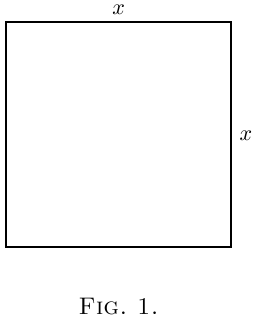
\includegraphics{018a.png}
\end{image}

\begin{image}
  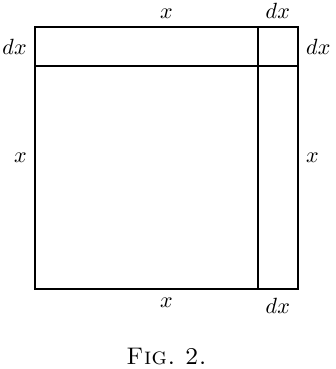
\includegraphics{019a.png}
\end{image}

Geometrically this may be depicted as follows: Draw a square (Figure
1) the side of which we will take to represent $x$. Now suppose the
square to grow by having a bit $dx$ added to its size each way. The
enlarged square is made up of the original square $x^2$, the two
rectangles at the top and on the right, each of which is of area $x
\cdot dx$ (or together $2x \cdot dx$), and the little square at the
top right-hand corner which is $(dx)^2$. In Figure 2 we have taken
$dx$ as quite a big fraction of $x$---about $\frac{1}{5}$. But suppose
we had taken it only $\frac{1}{100}$---about the thickness of an inked
line drawn with a fine pen. Then the little corner square will have an
area of only $\frac{1}{10,000}$ of $x^2$, and be practically
invisible. Clearly $(dx)^2$ is negligible if only we consider the
increment $dx$ to be itself small enough.


\begin{image}
  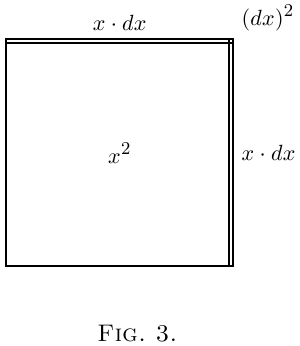
\includegraphics{019b.png}
\end{image}


Let us consider a simile.

Suppose a millionaire were to say to his secretary: next week I will
give you a small fraction of any money that comes in to me. Suppose
that the secretary were to say to his boy: I will give you a small
fraction of what I get. Suppose the fraction in each case to be
$\frac{1}{100}$ part. Now if Mr. Millionaire received during the next
week £$1000$, the secretary

would receive \pounds$10$ and the boy $2$ shillings. Ten
pounds would be a small quantity compared with
£$1000$; but two shillings is a small small quantity
indeed, of a very secondary order. But what would
be the disproportion if the fraction, instead of being $\frac{1}{100}$,
had been settled at $\frac{1}{1000}$ part? Then, while
Mr. Millionaire got his £$1000$, Mr. Secretary would
get only \pounds$1$, and the boy less than one farthing!

The witty Dean Swift once wrote:

\begin{quote}
So, Nat'ralists observe, a Flea Hath smaller Fleas that on him prey.
And these have smaller Fleas to bite 'em, And so proceed ad
infinitum.

\hfill On Poetry: a Rhapsody (p. 20), printed 1733---usually
misquoted.
\end{quote}

An ox might worry about a flea of ordinary size---a small creature of
the first order of smallness.  But he would probably not trouble
himself about a flea's flea; being of the second order of smallness,
it would be negligible. Even a gross of fleas' fleas would not be of
much account to the ox.

\end{document}
